\documentclass[11pt,border=20pt]{standalone}
\usepackage{tikz}
\usetikzlibrary{shapes.geometric, arrows.meta, positioning, shadows, patterns, decorations.pathreplacing, calc, fit, backgrounds, shapes.multipart}

% Define colors
\definecolor{frontend}{RGB}{66, 165, 245}
\definecolor{backend}{RGB}{255, 167, 38}
\definecolor{python}{RGB}{76, 175, 80}
\definecolor{data}{RGB}{156, 39, 176}
\definecolor{websocket}{RGB}{255, 87, 34}
\definecolor{phase}{RGB}{33, 150, 243}
\definecolor{darkgray}{RGB}{66, 66, 66}

% Define styles
\tikzstyle{component} = [rectangle, rounded corners, minimum width=2.8cm, minimum height=0.9cm, text centered, draw=black, line width=0.8pt, font=\sffamily\footnotesize]
\tikzstyle{frontend_comp} = [component, fill=frontend!20, draw=frontend!70]
\tikzstyle{backend_comp} = [component, fill=backend!20, draw=backend!70]
\tikzstyle{python_comp} = [component, fill=python!20, draw=python!70]
\tikzstyle{data_comp} = [component, fill=data!20, draw=data!70]
\tikzstyle{phase_box} = [rectangle, rounded corners, minimum width=3cm, minimum height=0.8cm, text centered, draw=phase!70, fill=phase!10, font=\sffamily\small]
\tikzstyle{arrow} = [thick,->,>=stealth, darkgray]
\tikzstyle{biarrow} = [thick,<->,>=stealth, darkgray]
\tikzstyle{websocket_arrow} = [thick,->,>=stealth, websocket, dashed]
\tikzstyle{label} = [font=\sffamily\tiny, darkgray]
\tikzstyle{title} = [font=\sffamily\Large\bfseries, darkgray]
\tikzstyle{subtitle} = [font=\sffamily\normalsize\bfseries, darkgray]
\tikzstyle{endpoint} = [rectangle, rounded corners, minimum width=2.5cm, minimum height=0.5cm, text centered, draw=backend!70, fill=backend!10, font=\sffamily\tiny]

\begin{document}
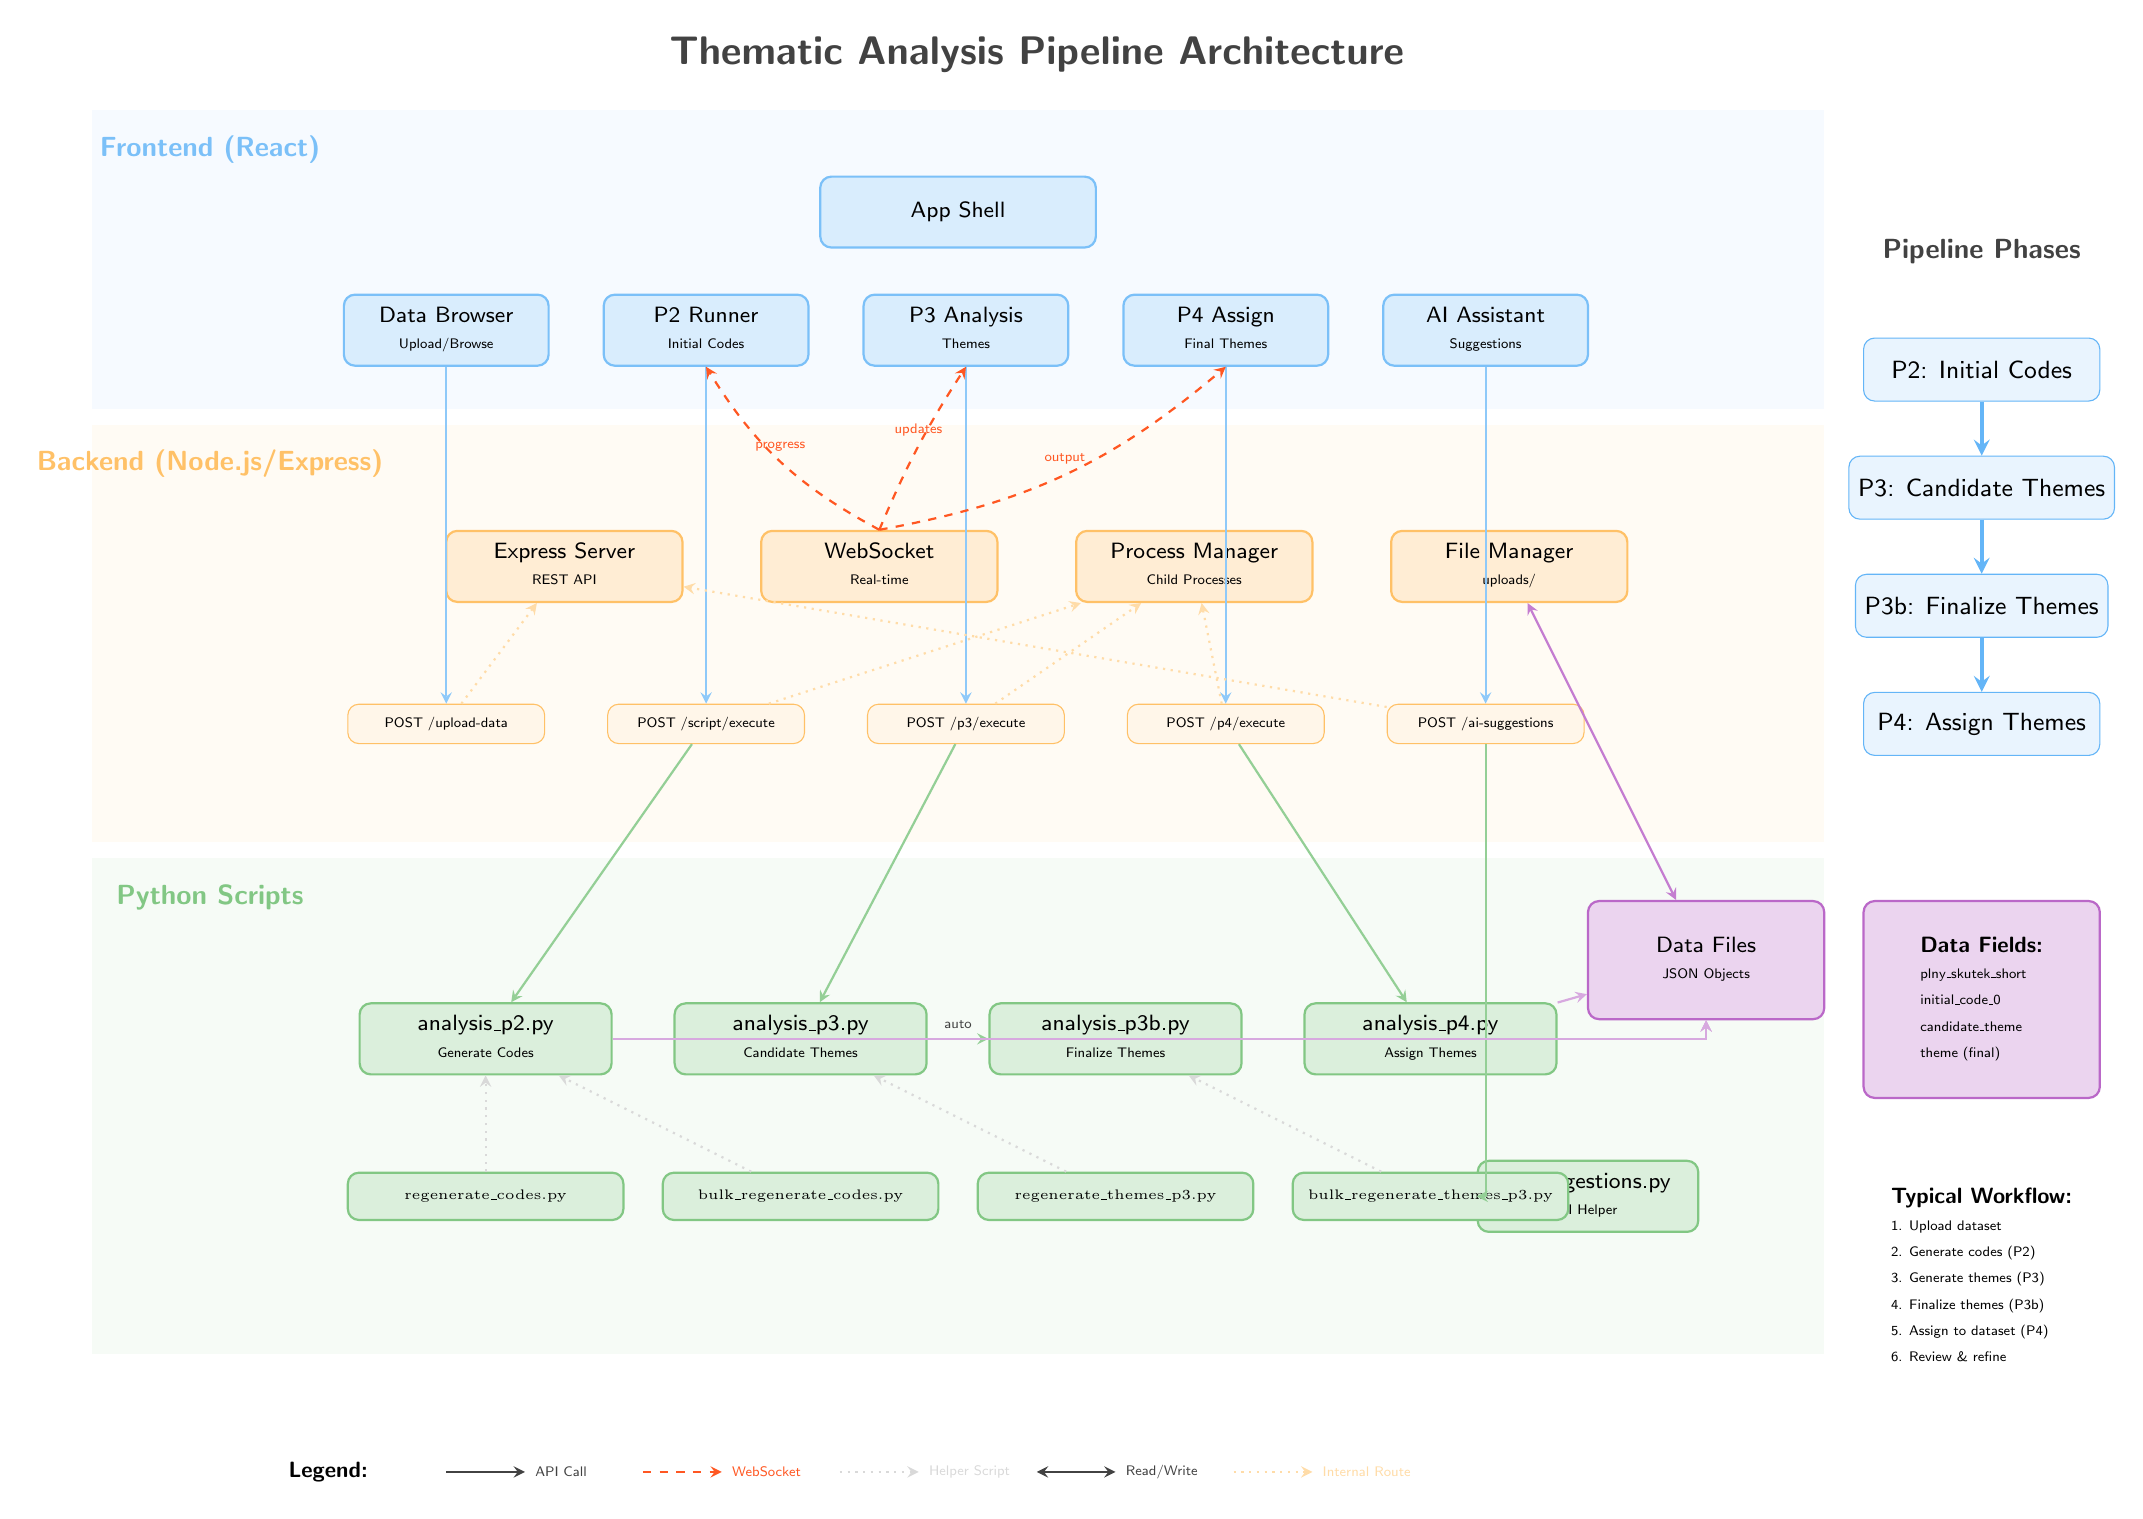
\begin{tikzpicture}[scale=1, transform shape]

% Title
\node[title] at (10, 16.5) {Thematic Analysis Pipeline Architecture};

% Architecture Layers - adjusted sizes
\begin{scope}[on background layer]
    \fill[frontend!5] (-2, 12) rectangle (20, 15.8);
    \fill[backend!5] (-2, 6.5) rectangle (20, 11.8);
    \fill[python!5] (-2, 0) rectangle (20, 6.3);
\end{scope}

% Layer Labels
\node[subtitle, frontend!70] at (-0.5, 15.3) {Frontend (React)};
\node[subtitle, backend!70] at (-0.5, 11.3) {Backend (Node.js/Express)};
\node[subtitle, python!70] at (-0.5, 5.8) {Python Scripts};

% Frontend Components - better spacing
\node[frontend_comp, minimum width=3.5cm] (app) at (9, 14.5) {App Shell};

\node[frontend_comp, minimum width=2.6cm] (browser) at (2.5, 13) {\begin{tabular}{c}Data Browser\\{\tiny Upload/Browse}\end{tabular}};
\node[frontend_comp, minimum width=2.6cm] (p2ui) at (5.8, 13) {\begin{tabular}{c}P2 Runner\\{\tiny Initial Codes}\end{tabular}};
\node[frontend_comp, minimum width=2.6cm] (p3ui) at (9.1, 13) {\begin{tabular}{c}P3 Analysis\\{\tiny Themes}\end{tabular}};
\node[frontend_comp, minimum width=2.6cm] (p4ui) at (12.4, 13) {\begin{tabular}{c}P4 Assign\\{\tiny Final Themes}\end{tabular}};
\node[frontend_comp, minimum width=2.6cm] (ai) at (15.7, 13) {\begin{tabular}{c}AI Assistant\\{\tiny Suggestions}\end{tabular}};

% Backend Main Components - better spacing
\node[backend_comp, minimum width=3cm] (server) at (4, 10) {\begin{tabular}{c}Express Server\\{\tiny REST API}\end{tabular}};
\node[backend_comp, minimum width=3cm] (ws) at (8, 10) {\begin{tabular}{c}WebSocket\\{\tiny Real-time}\end{tabular}};
\node[backend_comp, minimum width=3cm] (proc) at (12, 10) {\begin{tabular}{c}Process Manager\\{\tiny Child Processes}\end{tabular}};
\node[backend_comp, minimum width=3cm] (files) at (16, 10) {\begin{tabular}{c}File Manager\\{\tiny uploads/}\end{tabular}};

% Backend Endpoints - positioned lower and spread out
\node[endpoint] (upload) at (2.5, 8) {POST /upload-data};
\node[endpoint] (execute) at (5.8, 8) {POST /script/execute};
\node[endpoint] (p3exec) at (9.1, 8) {POST /p3/execute};
\node[endpoint] (p4exec) at (12.4, 8) {POST /p4/execute};
\node[endpoint] (aiapi) at (15.7, 8) {POST /ai-suggestions};

% Python Scripts - main analysis scripts
\node[python_comp, minimum width=3.2cm] (p2py) at (3, 4) {\begin{tabular}{c}analysis\_p2.py\\{\tiny Generate Codes}\end{tabular}};
\node[python_comp, minimum width=3.2cm] (p3py) at (7, 4) {\begin{tabular}{c}analysis\_p3.py\\{\tiny Candidate Themes}\end{tabular}};
\node[python_comp, minimum width=3.2cm] (p3bpy) at (11, 4) {\begin{tabular}{c}analysis\_p3b.py\\{\tiny Finalize Themes}\end{tabular}};
\node[python_comp, minimum width=3.2cm] (p4py) at (15, 4) {\begin{tabular}{c}analysis\_p4.py\\{\tiny Assign Themes}\end{tabular}};

% AI suggestions script
\node[python_comp, minimum width=2.8cm] (aipy) at (17, 2) {\begin{tabular}{c}ai\_suggestions.py\\{\tiny AI Helper}\end{tabular}};

% Regeneration Scripts - positioned lower with better spacing
\node[python_comp, minimum width=3.5cm, minimum height=0.6cm, font=\tiny] (regen1) at (3, 2) {regenerate\_codes.py};
\node[python_comp, minimum width=3.5cm, minimum height=0.6cm, font=\tiny] (regen2) at (7, 2) {bulk\_regenerate\_codes.py};
\node[python_comp, minimum width=3.5cm, minimum height=0.6cm, font=\tiny] (regen3) at (11, 2) {regenerate\_themes\_p3.py};
\node[python_comp, minimum width=3.5cm, minimum height=0.6cm, font=\tiny] (regen4) at (15, 2) {bulk\_regenerate\_themes\_p3.py};

% Data Storage - moved to avoid overlap
\node[data_comp, minimum width=3cm, minimum height=1.5cm] (data) at (18.5, 5) {\begin{tabular}{c}Data Files\\{\tiny JSON Objects}\end{tabular}};

% Pipeline Flow - adjusted position
\node[subtitle] at (22, 14) {Pipeline Phases};
\node[phase_box] (phase1) at (22, 12.5) {P2: Initial Codes};
\node[phase_box] (phase2) at (22, 11) {P3: Candidate Themes};
\node[phase_box] (phase3) at (22, 9.5) {P3b: Finalize Themes};
\node[phase_box] (phase4) at (22, 8) {P4: Assign Themes};

% Phase arrows
\draw[arrow, line width=1.5pt, phase!70] (phase1) -- (phase2);
\draw[arrow, line width=1.5pt, phase!70] (phase2) -- (phase3);
\draw[arrow, line width=1.5pt, phase!70] (phase3) -- (phase4);

% Data fields annotation - repositioned
\node[data_comp, minimum width=3cm, minimum height=2.5cm] (fields) at (22, 4.5) {
    \begin{tabular}{l}
    \textbf{Data Fields:}\\
    {\tiny plny\_skutek\_short}\\
    {\tiny initial\_code\_0}\\
    {\tiny candidate\_theme}\\
    {\tiny theme (final)}
    \end{tabular}
};

% Typical Workflow - repositioned
\node[align=left, font=\sffamily\footnotesize] at (22, 1) {
    \textbf{Typical Workflow:}\\
    {\tiny 1. Upload dataset}\\
    {\tiny 2. Generate codes (P2)}\\
    {\tiny 3. Generate themes (P3)}\\
    {\tiny 4. Finalize themes (P3b)}\\
    {\tiny 5. Assign to dataset (P4)}\\
    {\tiny 6. Review \& refine}
};

% Connections - Frontend to Endpoints
\draw[arrow, frontend!60] (browser) -- (upload);
\draw[arrow, frontend!60] (p2ui) -- (execute);
\draw[arrow, frontend!60] (p3ui) -- (p3exec);
\draw[arrow, frontend!60] (p4ui) -- (p4exec);
\draw[arrow, frontend!60] (ai) -- (aiapi);

% Endpoints to Backend components
\draw[arrow, backend!40, dotted] (upload) -- (server);
\draw[arrow, backend!40, dotted] (execute) -- (proc);
\draw[arrow, backend!40, dotted] (p3exec) -- (proc);
\draw[arrow, backend!40, dotted] (p4exec) -- (proc);
\draw[arrow, backend!40, dotted] (aiapi) -- (server);

% WebSocket connections - better routing
\draw[websocket_arrow, bend left=15] (ws.north) to node[above, label, websocket] {progress} (p2ui.south);
\draw[websocket_arrow, bend left=5] (ws.north) to node[above, label, websocket] {updates} (p3ui.south);
\draw[websocket_arrow, bend right=15] (ws.north) to node[above, label, websocket] {output} (p4ui.south);

% Backend to Python
\draw[arrow, python!60] (execute) -- (p2py);
\draw[arrow, python!60] (p3exec) -- (p3py);
\draw[arrow, python!60] (p3py) -- node[above, label] {auto} (p3bpy);
\draw[arrow, python!60] (p4exec) -- (p4py);
\draw[arrow, python!60] (aiapi) |- (aipy);

% Data connections
\draw[biarrow, data!60] (files) -- (data);
\draw[arrow, data!40] (p2py) -| (data);
\draw[arrow, data!40] (p3py) -| (data);
\draw[arrow, data!40] (p3bpy) -| (data);
\draw[arrow, data!40] (p4py) -- (data);

% Regeneration connections
\draw[arrow, gray!30, dotted] (regen1) -- (p2py);
\draw[arrow, gray!30, dotted] (regen2) -- (p2py);
\draw[arrow, gray!30, dotted] (regen3) -- (p3py);
\draw[arrow, gray!30, dotted] (regen4) -- (p3bpy);

% Legend - repositioned at bottom
\begin{scope}[shift={(1, -1.5)}]
    \node[font=\sffamily\footnotesize\bfseries] at (0, 0) {Legend:};
    \draw[arrow] (1.5, 0) -- (2.5, 0) node[right, font=\sffamily\tiny] {API Call};
    \draw[websocket_arrow] (4, 0) -- (5, 0) node[right, font=\sffamily\tiny] {WebSocket};
    \draw[arrow, gray!30, dotted] (6.5, 0) -- (7.5, 0) node[right, font=\sffamily\tiny] {Helper Script};
    \draw[biarrow] (9, 0) -- (10, 0) node[right, font=\sffamily\tiny] {Read/Write};
    \draw[arrow, backend!40, dotted] (11.5, 0) -- (12.5, 0) node[right, font=\sffamily\tiny] {Internal Route};
\end{scope}

\end{tikzpicture}
\end{document}